% Sångtext till VN:s sångbok 2018.

% Denna fil kan användas som sådan, bara verserna,
% namnen och annan rådata behöver bytas ur fälten.
% Tecknet "%" markerar en kommentar som helt och 
% hållet ignoreras av programmet som läser filen.

\beginsong{Djungelpunsch}[ 		% Börja sången här
	by={},					% Författare
	sr={Var nöjd med allt som livet ger},					% Melodi
	index={Jag gillar alla tiders punsch}]						% sång 



\beginverse*						% Börja vers
Jag gillar alla tiders punsch.
Punsch till frukost, punsch till lunch,
en punsch till förrätt, varmrätt och dessert.
Jag gillar punsch för vet du vad,
rent kaffe gör ju ingen glad.
Så punsch för fulla muggar vill jag ha.
\endverse							% Sluta vers

\beginverse*						% Börja vers
Med konjak du lockar.
Den bästa Renault.
Förlåt om jag chockar
och tar punsch ändå.
Och bjuder du på fin likör
får du ursäkta om det stör.
Jag väljer hellre Grönstedts Blå,
en Cederlunds eller Flaggpunsch å
- kanske har du ren Platin?
\endverse							% Sluta vers

\beginverse*						% Börja vers
Jag gillar punsch,
så ge mig punsch och jag är din.
/: För evigt din:/
\endverse							% Sluta vers

\endsong							% Sluta sång

\begin{intersong}
	\begin{center}
		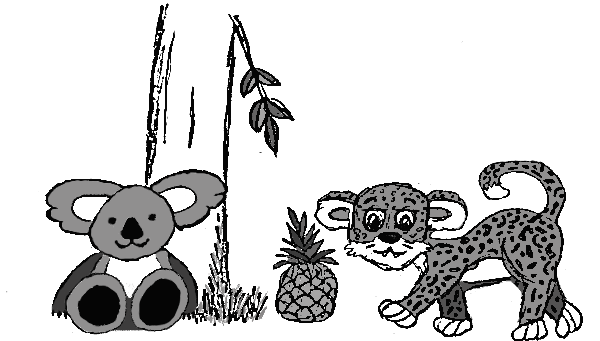
\includegraphics[width=0.7\textwidth]{../bilder/fardigabilder/CamillasFardigaBilder/Djungelboken2.png} 
	\end{center}
\end{intersong}
